{Terminata la breve parentesi teorica introduttiva,  si procede in questo capitolo alla presentazione
dell'impostazione pratica che si è voluto dare alle sperimentazioni condotte. La struttura secondo cui
saranno esposte le informazioni nei seguenti paragrafi ricalca la partizione logica alla base del codice
sviluppato, pragmaticamente diviso in quattro moduli tra loro indipendenti:}

\begin{itemize}
\item generazione dei grafi
\item generazione delle istanze di problemi MIP
\item risoluzione delle istanze di problemi MIP
\item estrazione ed analisi dei dati
\end{itemize}

\section{Generazione dei grafi}
L'iniziale problema che è stato necessario affrontare nello svolgimento di questo lavoro è stata la 
generazione automatica e pseudo-casuale di grafi, indispensabile al fine di ottenere un numero sufficiente di 
istanze da cui estrarre informazioni statisticamente rilevanti. Quello della generazione di grafi pseudo-casuali è un problema noto in letteratura, in quanto in numerosi ambiti di ricerca, che spaziano dalla biologia 
molecolare allo studio delle reti di calcolatori, si rende necessaria la generazione casuale di queste strutture 
dati nello studio delle realtà di loro interesse. 
Di conseguenza, nel corso degli ultimi decenni sono stati molti i metodi proposti dalla comunità scientifica al 
fine di affrontare il problema. Tra questi ne sono stati selezionati quattro, sulla base delle proprietà e delle caratteristiche particolari di ciascuno di essi.  

La gestione dei grafi a livello di codice è stata implementata utilizzando NetworkX, una libreria stabile e flessibile sviluppata appositamente per lo studio e la rappresentazione di grafi in Python \cite{networkx}. NetworkX offre, oltre alla possibilità di rappresentazione, diversi algoritmi per lo studio delle proprietà e il calcolo di determinate misure su istanze di grafi fornite. La libreria comprende inoltre inoltre un insieme di metodi che implementano un gran numero di modelli standard noti in letteratura per la generazione di grafi, tra cui naturalmente quelli utilizzati in questo lavoro. 

Inoltre, tutti i grafi generati in questo lavoro sono stati salvati sotto forma di \textit{adjacency list}, in modo tale da poter essere letti ed elaborati da altri moduli del programma a posteriori. Il salvataggio è stato svolto mediante un apposito metodo della libreria,  \texttt{write\_adjlist(G, path)}. In una lista di adiacenze ogni nodo è rappresentato da una stringa nel formato
\vspace{-0.6cm}
\begin{equation*}
\verb|nodo [vicino] [vicino] ... [vicino]|
\end{equation*}

\subsection{Modello di Erdős–Rényi}
\label{subsec:er}
Il modello di Erdős–Rényi è un modello per la generazione di grafi casuali, detti grafi Erdős–Rényi (\textsl{ER}) o binomiali, introdotto per la prima volta nel 1959 dai matematici ungheresi Paul Erdős e Alfréd Rényi \cite{erdos59a}. 
Nella formulazione $G(n,p)$ del modello,  un grafo di $n$ nodi viene costruito secondo un procedimento iterativo, in cui ogni arco tra due nodi del grafo viene generato con una probabilità $p$ fissata ed indipendentemente da quella con cui sono generati gli altri archi.  

Formalmente, un grafo ER, anche detto $G(n,p)$, è un grafo (N,G) con $N={1,2,\dots n}$ insieme dei nodi e in cui la matrice delle adiacenze G = $(g_{ij})$ è tale per cui, per ogni coppia di nodi distinti $i$ e $j$, la probabilità che $g_{ij} = 1$ è $P(g_{ij}=1)=p$, con $p \in [0,1]$. 

I parametri di questo modello sono quindi due, il numero di nodi del grafo $n$ e la probabilità di generazione di ogni arco $p$.  A parità di parametri, i grafi che si possono ottenere sono in ogni caso molti, come mostrato in Figura \ref{fig:gnpes}. 

\begin{figure}[h!]
     \centering
     \begin{subfigure}[b]{0.29\textwidth}
         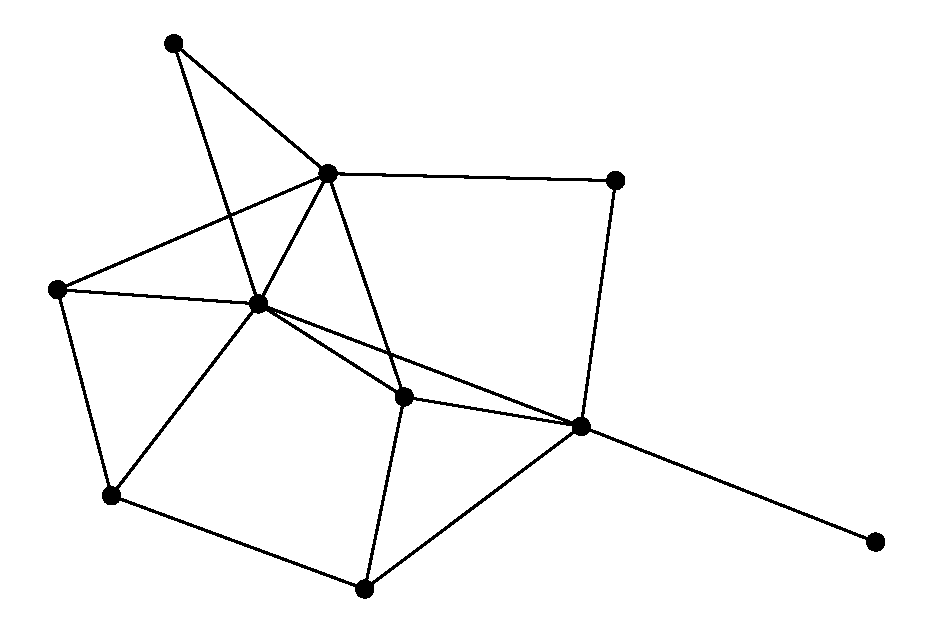
\includegraphics[width=\columnwidth]{images/gnpes2.eps}
     \end{subfigure}
     \hspace{0.8em}
     \begin{subfigure}[b]{0.29\textwidth}
         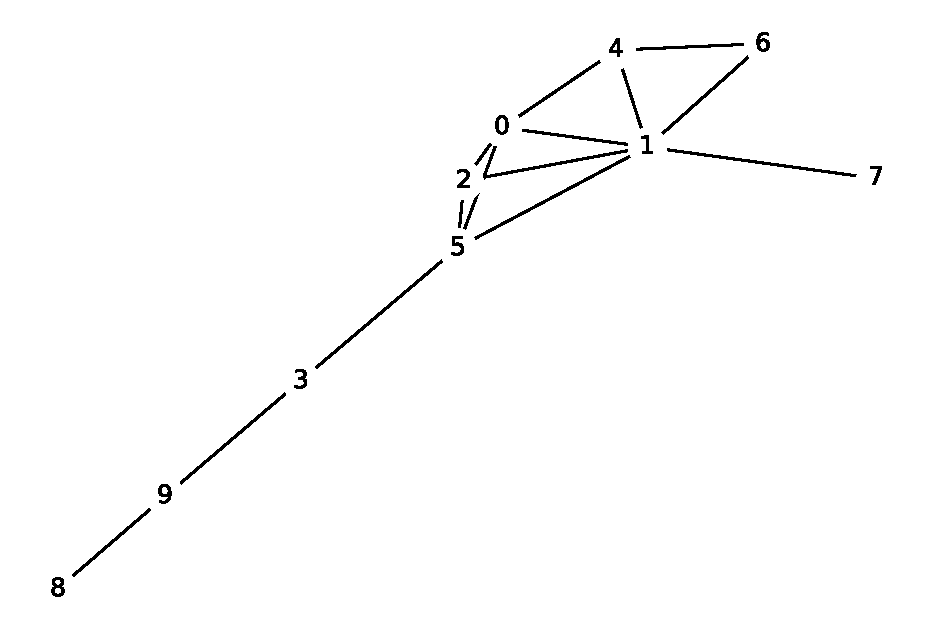
\includegraphics[width=\columnwidth]{images/gnpes1.eps}
     \end{subfigure}
     \hspace{0.8em}
     \begin{subfigure}[b]{0.29\textwidth}
         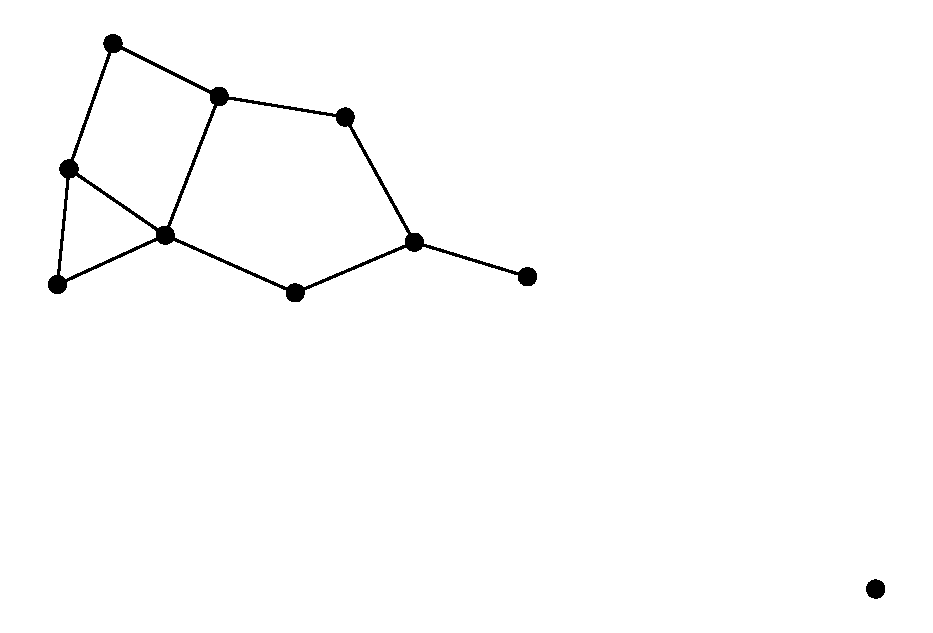
\includegraphics[width=\columnwidth]{images/gnpes0.eps}
     \end{subfigure}
        \caption{Diversi grafi $G(n,p)$ generati a partire dagli stessi parametri $n=10$ e $p=0.3$ con la libreria NetworkX e visualizzati graficamente con l'ausilio di un'altra libreria Python, Matplotlib \cite{Hunter2007}.}
        \label{fig:gnpes}
\end{figure}

Il metodo di NetworkX utilizzato nella generazione di questa tipologia di grafi è \linebreak
\texttt{gnp\_random\_graph(n, p, seed)}, che restituisce un'istanza di grafo $G(n,p)$ di dimensione \texttt{n} in cui gli archi hanno probabilità di essere generati pari a \texttt{p}, mentre il parametro \texttt{seed} regola il comportamento pseudo-casuale, in modo tale da permettere la riproducibilità degli esperimenti. Lo pseudo-codice dell'algoritmo che gestisce la generazione di questa tipologia di grafi è riportato in Algoritmo \ref{alg:gnp}.

\begin{algorithm}
\SetAlgoLined
\KwIn{numero di nodi $n$ e probabilità di generazione di ogni arco $p$}
 inizializza il grafo vuoto $G$\;
 aggiungi i nodi $1 \dots n$ a $G$\;
 \ForEach{{\upshape coppia di nodi} e=(i,j)}{
 	$rand$ = numero casuale $\in [0,1]$\;
 	\If{rand $>$ p} {
 		aggiungi l'arco $e$ a $G$\;
 	}
 }
 \Return{$G$}
 \caption{Generazione di un grafo di Erdős–Rényi}
 \label{alg:gnp}
\end{algorithm}

Tuttavia, l'assunto principale su cui è basata la generazione in questo modello, ovvero che a tutti gli archi è associata una probabilità di generazione uguale ed indipendente da quella degli altri archi, potrebbe risultare poco veritiero nella generazione di grafi casuali il cui scopo è modellare certe categorie di fenomeni del mondo reale. Molte proprietà dei grafi nel mondo reale, infatti, non riescono ad essere replicate da questo particolare modello di generazione casuale.

Per questa ragione sono stati sviluppati nel corso del tempo diversi altri modelli di generazione basati su meccanismi completamente diversi, come ad esempio \textit{rewiring} e \textit{preferential-attachment}, di cui verranno presentati degli esempi più avanti. 

\subsection{Modello di Steger-Wormald}
\label{subsec:steger}
Nella teoria dei grafi, un grafo è detto \textit{regolare di grado} $d$ quando tutti i suoi vertici hanno lo stesso grado, ossia lo stesso numero di archi incidenti. Se tale grado comune è uguale a $d$, il grafo è detto $d$-regolare. Un grafo regolare casuale è un grafo selezionato da $\mathcal{G}_{n,r}$, lo spazio di probabilità di tutti i possibili grafi $r$-regolari di $n$ vertici, in cui $3\leq r < n$ e $nr$ è pari. In questo spazio ogni grafo $d$-regolare di $n$ nodi ha la stessa probabilità $\frac{1}{|\mathcal{G}_{n,r}|}$ di essere generato. Si tratta quindi di grafi random, le cui caratteristiche sono tuttavia significativamente diverse dal caso generale a causa del vincolo di regolarità.

Dal momento che la maggior parte dei grafi random (che possono essere generati ad esempio mediante il modello di Erdős–Rényi precedentemente esposto nella Sottosezione \ref{subsec:er}) non sono regolari, l'implementazione di un algoritmo imparziale per la generazione di grafi regolari casuali non è così scontata. 

Un modello tipicamente utilizzato per la generazione di grafi $d$-regolari con $d$ piccolo è il cosiddetto \textit{pairing model}. Tale modello si basa sulla definizione di $n$ insiemi, uno per ogni vertice del grafo da generare, contenenti ciascuno $d$ elementi, tanti quanti il numero di archi che devono incidere ogni nodo. La costruzione del grafo avviene quindi selezionando iterativamente due insiemi $i$ e $j$, con $i \neq j$ e per cui non esiste già un arco nel grafo che collega i due nodi corrispondenti, aggiungendo al grafo l'arco $(i,j)$ e rimuovendo dai corrispettivi insiemi un elemento ciascuno. 

Questo modello è molto intuitivo ma viene solitamente utilizzato nella generazione di istanze di grafi dove $d$ è molto piccolo, come già accennato in precedenza. Si può dimostrare infatti che la complessità computazionale dell'algoritmo è esponenziale nella grandezza di $d$, dell'ordine di $nde^{(d^2-1)/4}$ \cite{steger_wormald_1999} per valori di $d$ fino a $n^{\frac{1}{3}}$.

In questo lavoro la generazione dei grafi regolari random è stata quindi implementata utilizzando una versione ottimizzata del modello ad accoppiamento, proposta nel 1999 dai matematici Angelika Steger e Nick Wormald \cite{steger_wormald_1999}. Lo pseudo-codice dell'algoritmo utilizzato nel metodo proposto da questi ultimi è riportato in Algoritmo \ref{alg:rrg}. Alcuni esempi di grafi regolari random generati mediante il modello di Steger-Wormald sono riportati in Figura \ref{fig:rrges}.

\begin{figure}[h!]
     \centering
     \begin{subfigure}[b]{0.29\textwidth}
         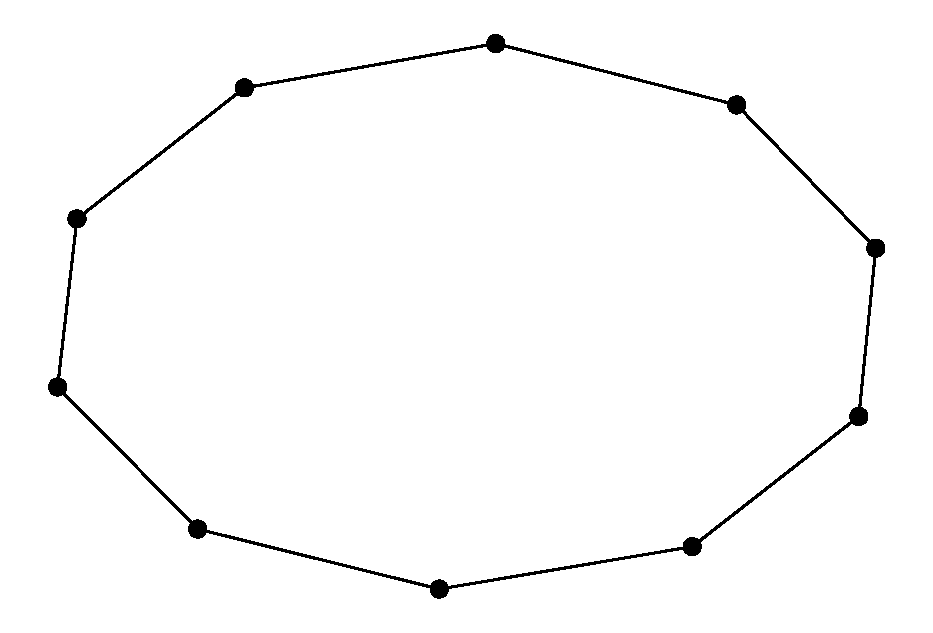
\includegraphics[width=\columnwidth]{images/rrges-1.eps}
     \end{subfigure}
     \hspace{0em}
     \begin{subfigure}[b]{0.29\textwidth}
         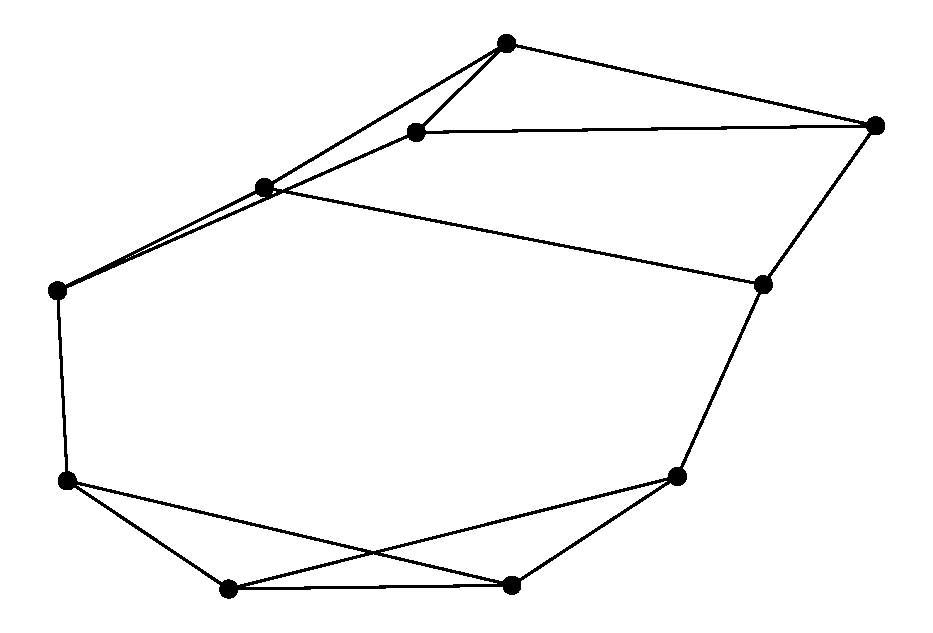
\includegraphics[width=\columnwidth]{images/rrges0.eps}
     \end{subfigure}
     \hspace{0em}
     \begin{subfigure}[b]{0.29\textwidth}
         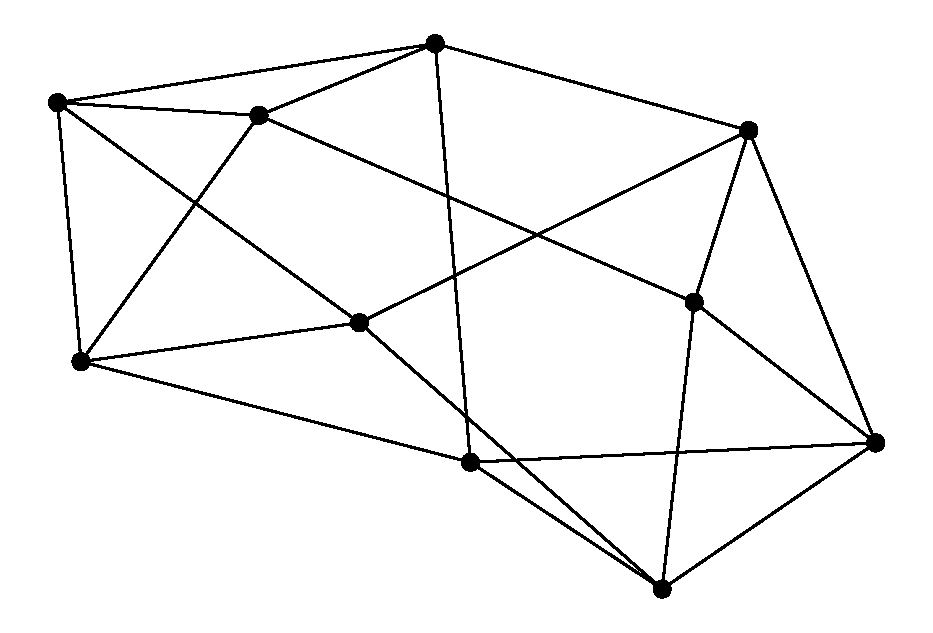
\includegraphics[width=\columnwidth]{images/rrges1.eps}
     \end{subfigure}
        \caption{Diversi grafi regolari di dimensione 10 generati utilizzando il metodo \texttt{random\_regular\_graph(d, n)} della libreria NetworkX con $d$ pari a, da sinistra verso destra,  $2$,$3$ e $4$.}
        \label{fig:rrges}
\end{figure}

Il metodo di NetworkX utilizzato nella generazione di questa tipologia di grafi è\\
\texttt{random\_regular\_graph(d, n, seed)}, che restituisce un'istanza di grafo regolare di dimensione \texttt{n} in cui tutti i nodi hanno grado \texttt{d}. Il parametro \texttt{seed} anche in questo caso regola il comportamento pseudo-casuale della generazione, permettendo la replicabilità dell'esperimento.

\begin{algorithm}
\SetKwRepeat{Do}{do}{while}
\SetAlgoLined
\KwIn{numero di nodi $n$ e numero di archi incidenti per ogni nodo $d$}
\Do{G {\upshape non è $d$-regolare}}{
	 inizializza un grafo $G$ con $n$ nodi e nessun vertice\;
	 inizializza un insieme $S$ di coppie di nodi non adiacenti e il cui grado è al massimo $d-1$\;
	 \Do{S {\upshape non è vuoto}}{
	 	assegna ad ogni coppia $(u,v)$ in $S$ una probabilità di essere scelta proporzionale a $(d-d(u))(d-d(v))$\;
	 	scegli una coppia $(u,v)$ da $S$ sulla base delle probabilità calcolate\;
	 	aggiungi l'arco $(u,v)$ a $g$\;
	 	rimuovi la coppia $u,v$ da S\;
	 }
 }
 \Return{$G$}
 \caption{Generazione di un grafo regolare con il modello di Steger-Wormald}
 \label{alg:rrg}
\end{algorithm}


\subsection{Modello di Watts-Strogatz}
Il modello di Watts-Strogatz è un modello per la generazione di grafi casuali presentato nel 1998 da Duncan J. Watts e Steven Strogatz \cite{watts_collective_1998}, la cui caratteristica principale risiede nel possedere proprietà \textit{small-world}. 

Il concetto di small-world venne introdotto per la prima volta nel 1967 dallo psicologo statunitense Stanley Milgram nella sua serie di esperimenti mirata ad esaminare la lunghezza media dei percorsi delle reti sociali tra residenti negli Stati Uniti (popolarmente conosciuti con il nome di "\textit{six degrees of separation}") \cite{milgram_small-world_1967}. In questi esperimenti Milgram ipotizzò l'aderenza dei contesti sociali da lui analizzati ad un modello a "\textit{piccolo mondo}", composto da una rete di collegamenti tra persone relativamente breve.  

Watts e Strogatz, partendo dalle osservazioni di Milgram, verificarono che diversi esempi di grafi che rappresentano contesti reali, tra cui il sistema nervoso del verme nematode fasmidario \textit{Caenorhabditis elegans}, la rete elettrica degli Stati Uniti occidentali e un grafo rappresentante le collaborazioni tra diversi attori di film, mostrano alcune proprietà comuni molto importanti. Sulla base di queste osservazioni proposero quindi un modello di rete denominato \textit{small-world network}, caratterizzato da:
\begin{itemize}
\item lunghezza media del cammino minimo tra due nodi molto bassa
\item tendenza al raggruppamento in cluster all'interno della rete, che si traduce in regolarità e località del grafo
\end{itemize}

Nessuno dei principali metodi di generazione di grafi casuali garantiva tuttavia la generazione di grafi con tali caratteristiche. I grafi $G(n,p)$ infatti presentano caratteristiche simili a reti small-world, ma non hanno un alto coefficiente di clusterizzazione. Al contrario, i grafi regolari presentano un alto coefficiente di clusterizzazione ma lunghezza media dei cammini minimi generalmente elevata. 

Per questa ragione, Watts e Strogatz proposero un nuovo modello di generazione di grafi casuali,  basato su modifiche iterative di un grafo regolare ad anello mediante un \textit{rewiring} di archi del grafo controllato dal parametro $p$ (che modula la regolarità o, viceversa, la casualità del grafo prodotto, come mostrato in Figura \ref{fig:incwsg}). Queste modifiche consentono, per opportuni valori di $p$,  la conservazione di un alto livello di clustering locale ma, allo stesso tempo, abbattono la lunghezza del cammino minimo tra nodi del grafo mediante l'aggiunta di collegamenti casuali.  Un andamento di queste due proprietà al variare del valore di $p$ è riportato in Figura \ref{fig:lcwsg}. Lo pseudo-codice di questo metodo è riportato in Algoritmo \ref{alg:wsg}.


\begin{figure}[h!]
     \centering
     \begin{subfigure}[t]{7cm}
         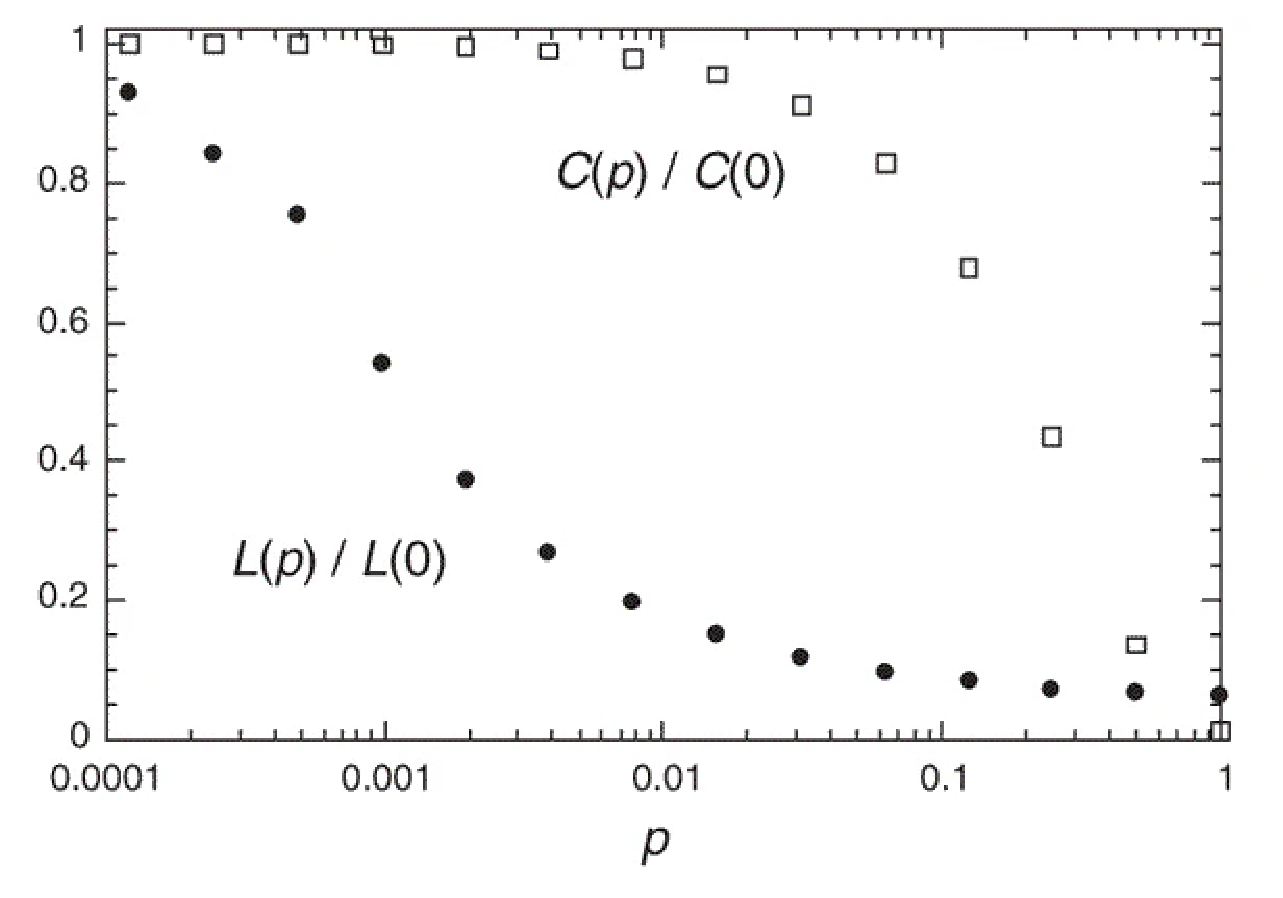
\includegraphics[width=\columnwidth]{images/wsgcl.eps}
         \caption{Clustering globale $C$ e lunghezza media del cammino minimo tra nodi $L$ al variare della probabilità di rewiring $p$.}
          \label{fig:lcwsg}
     \end{subfigure}
     \hspace{0.8em}
     \begin{subfigure}[t]{7cm}
     	\raisebox{0.9cm}{
         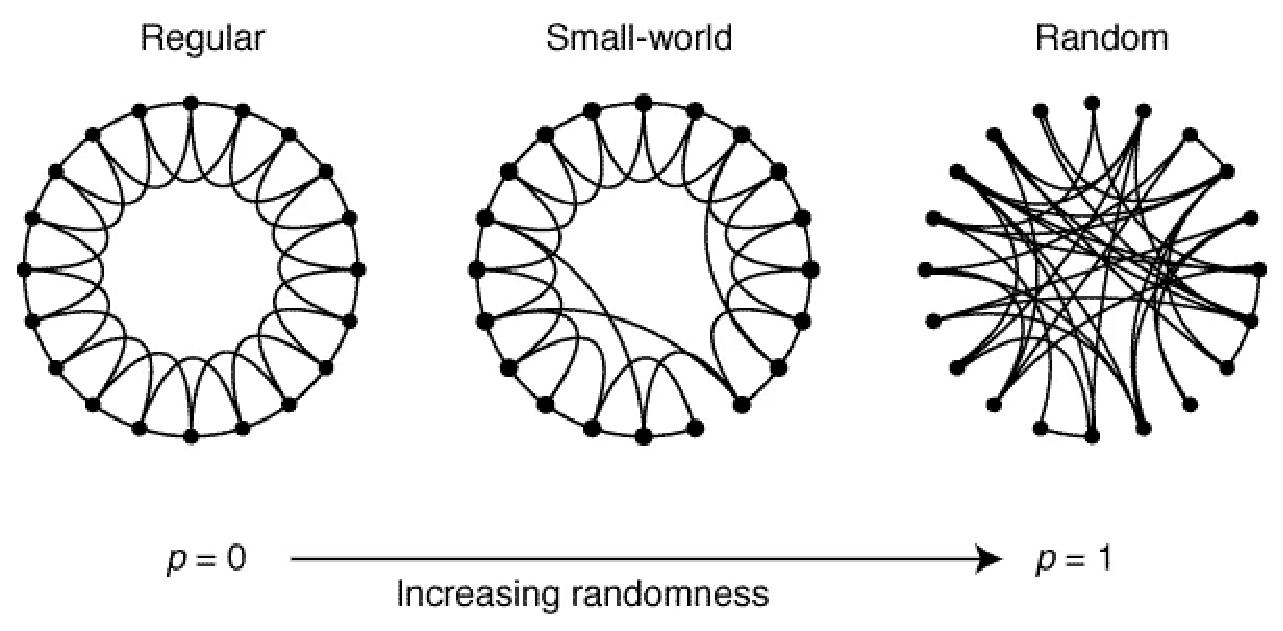
\includegraphics[width=\columnwidth]{images/wsginc.eps}}
         \caption{Regolarità del grafo in funzione della probabilità di rewiring $p$.}
          \label{fig:incwsg}
     \end{subfigure}
        \caption{Rappresentazioni grafiche che evidenziano caratteristiche proprie del modello di generazione proposto da Watts-Strogatz \cite{watts_collective_1998}.}
\end{figure}


Il metodo di NetworkX utilizzato nella generazione di questa tipologia di grafi è \linebreak
\texttt{watts\_strogatz\_graph(n, k, p, seed)}, che restituisce un'istanza di grafo di Watts-Strogatz di dimensione \texttt{n}. I nodi di questo grafo sono inizialmente organizzati in una struttura ad anello in cui ogni nodo è collegato ai suoi \texttt{k//2+1} vicini sinistri e \texttt{k//2+1} vicini destri ed in cui la probabilità che ciascun nodo sia "ricollegato" con un altro nodo diverso da uno dei suoi vicini attuali è \texttt{p}. Anche in questo caso il parametro \texttt{seed} regola il comportamento casuale della generazione, permettendo così di ottenere la riproducibilità dei risultati.

Questo modello di generazione presenta tuttavia diverse limitazioni. La principale tra queste riguarda il grado dei nodi che, a differenza della maggior parte dei grafi che rappresentano modelli reali, denota una varianza media molto bassa tra i nodi di uno stesso grafo. Inoltre, questo modello di generazione implica l'utilizzo di grafi con un numero fisso di nodi e, di conseguenza, non può essere utilizzato nella simulazione di realtà la cui dimensione è variabile nel tempo.

\begin{algorithm}
\SetAlgoLined
\KwIn{numero di nodi $n$, numero collegamenti iniziali con i vicini $k$ e probabilità di fare \textit{rewiring} di ciascun arco $p$}
 inizializza un grafo ad anello $G$ con $n$ nodi e nessun arco\;
 \ForEach{{\upshape nodo} m {\upshape appartenente al grafo}} {
 	aggiungi un arco tra $m$ e i suoi $k/2$ vicini destri e $k/2$ vicini sinistri\;
 }
 \ForEach{{\upshape arco} e=(u,v) {\upshape tra due nodi del grafo}}{
 	$rand$ = numero casuale $\in [0,1]$\;
 	\If{rand $>$ p} {
 		$w$ = nodo diverso da $v$ scelto casualmente con probabilità uniforme\;
 		$e = (u,w)$, ossia ricollega l'arco\;
 	}
 }
 \Return{$G$}
 \caption{Generazione di un grafo di Watts-Strogatz}
 \label{alg:wsg}
\end{algorithm}

\subsection{Modello di Barabási-Albert}
\label{subsec:barab}
Tutti i modelli visti fino a questo momento mancano di due aspetti fondamentali che caratterizzano invece i grafi reali. Per prima cosa, viene sempre assunta la presenza di un numero fisso di vertici nel grafo. Al contrario, molte delle delle reti nel mondo reale sono composte da un insieme di vertici che solitamente tende a crescere nel tempo. Alcuni esempi di grafi che hanno questo comportamento sono il World Wide Web, che cresce esponenzialmente con l'aggiunta di nuove pagine Web, e la letteratura scientifica, che cresce anch'essa nel tempo con la pubblicazione di nuovi articoli. 

In secondo luogo, nessuno dei modelli trattati in precedenza tiene conto del cosiddetto \textit{preferential attachment}, fenomeno per cui i nodi che si aggiungono alla rete sono solitamente più propensi a creare connessioni con nodi che hanno già un gran numero di connessioni con altri nodi. Ritornando agli esempi già citati del WWW e della letteratura scientifica, è più probabile che una nuova pagina Web includa link a pagine Web più conosciute e già referenziate da molte altre pagine, così come è molto probabile che un nuovo paper scientifico includa riferimenti ad altri paper influenti e già citati in molti altri lavori. 

Proprio sulla base di queste osservazioni i fisici Albert-László Barabási e Réka Albert proposero nel 1999 un nuovo modello per la generazione di grafi casuali \cite{Barab_si_1999}. Tale metodo è basato su di un meccanismo di \textit{preferential attachment}, in cui i nodi vengono aggiunti uno ad uno al grafo e la probabilità di creazione di un arco tra il nuovo nodo $i$ e uno di quelli esistenti $j$ dipende strettamente dal grado di quest'ultimo, secondo la relazione
\begin{align*}
p_i = \frac{k_i}{\sum_{j \in J}k_j}
\end{align*}
dove $J$ è l'insieme dei nodi già presenti nel grafo durante l'iterazione in cui viene aggiunto il nuovo nodo e $k_x$ corrisponde al numero di connessioni che incidono il nodo $x$ nella stessa iterazione. Lo pseudo-codice del modello di generazione è riportato in Algoritmo \ref{alg:bag}.

Il modello di Barabási-Albert ha quindi la capacità di generare un grafo con pochi nodi, detti \textit{hub}, che presentano un grado molto elevato se comparato a quello della maggior parte dei restanti nodi del grafo. 

Un'altra caratteristica molto importante dei grafi casuali generati utilizzando questo modello è quella di essere \textit{scale-free networks}, ovvero grafi per cui la relazione tra numero di nodi e numero di connessioni è di tipo esponenziale negativo, e quindi invariante ai cambiamenti di scala. 
Un confronto tra la distribuzione del grado dei nodi in un grafo $G(n,p)$ e in un grafo \textit{scale-free} è riportato di seguito in Figura \ref{fig:bagdist}. 

\begin{figure}[h!]
     \centering
       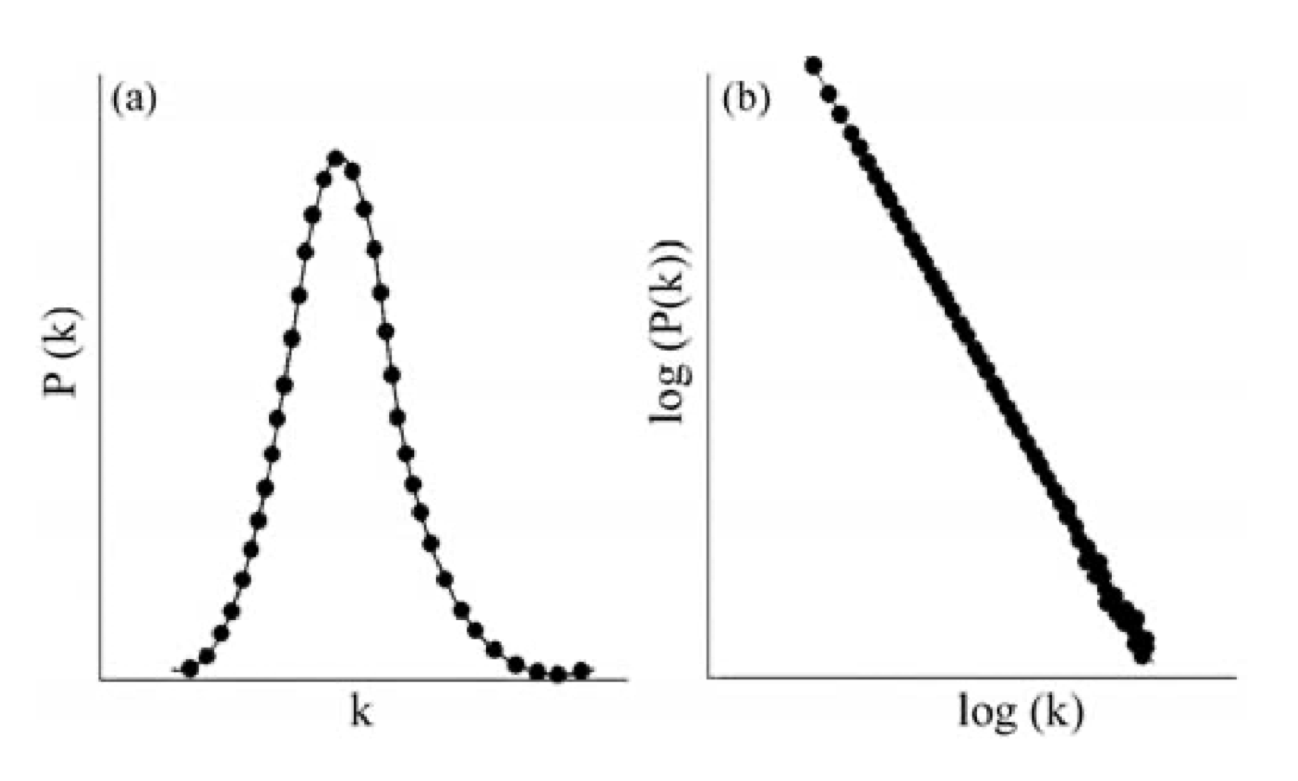
\includegraphics[scale=0.45]{images/bagdist.eps}
       \caption{Confronto tra la distribuzione del grado dei nodi in un grafo $G(n,p)$ (a sinistra)e in un grafo scale-free (a destra) \cite{costa}.}
        \label{fig:bagdist}
\end{figure}

A livello pratico, questo significa che confrontando il numero di due tipi di nodi, ad esempio quelli di grado $5$ e $15$, il rapporto tra i due risulta essere pari a
\begin{align*}
e^{-a(Nb-Na)}
\end{align*}
dove $Na$ e $Nb$ sono rispettivamente il numero di nodi del denominatore e del numeratore mentre $a$ è un parametro del tipo di rete considerato.

Il metodo di NetworkX utilizzato nella generazione di questa tipologia di grafi è\\
\texttt{barabasi\_albert\_graph(n, m, seed)}, che restituisce un'istanza di grafo Barabási-Albert di dimensione \texttt{n} in cui ogni nuovo nodo viene collegato nel procedimento iterativo a \texttt{m} nodi esistenti. Anche in questo caso il parametro \texttt{seed} regola il comportamento casuale della generazione, agendo in particolare sulla scelta dell'insieme di archi da creare ad ogni iterazione, permettendo così la replicabilità dell'esperimento. 

\begin{algorithm}
\SetAlgoLined
\KwIn{numero di nodi $n$ e numero di archi $m$ da creare tra ogni nuovo nodo ed i nodi esistenti}
 inizializza un grafo $G$ con $m$ nodi\;
 $target$ = lista inizialmente contenente gli $m$ nodi iniziali\;
 $r$ = lista di nodi inizialmente vuota\;
 \While{{\upshape ci sono ancora nodi da aggiungere}}{
 	aggiungi un nuovo nodo al grafo\;
 	genera un arco tra il nuovo nodo e ogni nodo in $target$\;
 	aggiungi il nuovo nodo $m$ volte a $r$\;
 	aggiungi tutti i nodi contenuti in $target$ a $r$\;
 	$target$ = sottoinsieme casuale di $r$ di cardinalità $m$\;
 }
 \Return{$G$}
 \caption{Generazione di un grafo di Barabási-Albert}
 \label{alg:bag}
\end{algorithm}

Sebbene rappresenti molto fedelmente per certi aspetti grafi reali, grazie soprattutto alla proprietà dell'invarianza di scala, il modello di generazione proposto da Barabási ed Albert non riesce a replicare altrettanto bene altre proprietà di queste reti, come ad esempio l'alto indice di clustering globale (proprietà che, al contrario, viene ricreata perfettamente dal modello di Watts-Strogatz). Per questo motivo sia il modello di Watts-Strogatz che quello di Barabási-Albert devono essere considerati come modelli solo parzialmente realistici.

%----------------------------------NEW SECTION
\newpage
\section{Generazione delle istanze di problemi MIP}
Terminata la generazione dei grafi, costituenti il \textit{dataset} grezzo alla base di questo lavoro, è stato necessario ricavare a partire da ciascuno di essi il corrispondente problema di programmazione lineare intera del vertex cover minimo. Per fare questo è stato inizialmente necessario ricavare una modellazione algebrica del problema stesso, definendo variabili, vincoli e funzione obiettivo con cui rappresentarlo formalmente. Solo in un secondo momento è stato quindi possibile procedere con l'implementazione del modello nel software e la costruzione delle singole istanze, mediante l'ausilio di un'apposita libreria Python.

\subsection{Modellazione algebrica}
Un \textit{modello algebrico} di un problema di programmazione lineare intera è un modello che descrive le caratteristiche della soluzione ottima al problema mediante relazioni matematiche \cite{rop}. Un modello algebrico è composto dai seguenti elementi:
\begin{itemize}
\item \textsl{insiemi}, che raggruppano gli elementi del sistema permettendo l'indicizzazione delle grandezze trattate nel problema
\item \textsl{parametri}, ossia quantità costanti e definite dalla formulazione del problema stesso, che solitamente sono delle proprietà degli insiemi precedentemente definiti
\item \textsl{variabili}, ossia le grandezze incognite del sistema, su cui l'algoritmo può agire (nei limiti dei vincoli imposti dal loro dominio) per ottimizzare il valore della soluzione
\item \textsl{vincoli}, ossia relazioni matematiche che permettono di verificare l'ammissibilità delle soluzioni e, di conseguenza, definire quali assegnazioni alle variabili sono accettabili nel contesto del problema e quali invece non lo sono
\item \textsl{funzione obiettivo}, che permette la traduzione di una soluzione del problema in un valore numerico, rendendone possibile di conseguenza l'ottimizzazione
\end{itemize}

Un modello algebrico di un problema di programmazione lineare permette quindi la definizione in forma dichiarativa delle caratteristiche della soluzione cercata, piuttosto che definire una strategia con cui eseguire la ricerca della soluzione stessa. Un modello di programmazione matematica potrebbe essere quindi paragonato ad un linguaggio dichiarativo, che descrive il risultato che si vuole ottenere, piuttosto che ad un linguaggio procedurale, che indica invece la sequenza di passi da percorrere per arrivare a quel risultato.

Durante la fase di modellazione formale del problema viene persa parte della potenza descrittiva caratteristica del linguaggio naturale, a vantaggio però della possibilità di utilizzare algoritmi particolarmente efficienti nella risoluzione dello stesso, che possono essere applicati solo quando il problema è definito in questa forma.

La modellazione algebrica non è stata, nel caso del problema analizzato in questo lavoro, particolarmente onerosa.

\noindent
Per prima cosa sono stati identificati gli insiemi del problema, ovvero
\begin{align*}
V \,  : \, \mbox{insieme dei vertici del grafo}\\
E \, : \, \mbox{insieme degli archi del grafo}
\end{align*}
Successivamente, è stato necessario identificare i parametri del problema. Avendo studiato la formulazione \textit{unweighted} del problema di vertex cover, in cui tutti i vertici hanno un peso associato $c_v=1$, non è stato necessario definire alcun parametro.  Infine sono state definite le variabili del problema, indicizzate dall'insieme dei vertici $V$
\begin{align*}
x_v = \begin{cases}  1 & \mbox{se il vertice } v \in V \mbox{ è compreso nel vertex cover} \\ 0 & \mbox{altrimenti} \end{cases}
\end{align*}
In questo caso il vincolo imposto dal problema è uno solo, ossia che almeno uno dei due vertici collegati da un arco sia presente nel vertex cover, per ognuno degli archi del grafo. Questo vincolo può essere rappresentato in forma dichiarativa mediante le variabili e gli insiemi precedentemente definiti come
\begin{align*}
x_u + x_v \geq 1 \quad \forall (u,v) \in E,  u \in V, v \in V
\end{align*}
La definizione della funzione obiettivo $f(x)$, che dovrà essere minimizzata dal risolutore,  viene a questo punto naturale
\vspace{-0.5cm}
\begin{align*}
f(x) = \sum_{v \in V} x_v
\end{align*}
Il modello algebrico del problema di programmazione lineare del minimo vertex cover può quindi essere complessivamente definito come 
\begin{align}
    \label{eq:mipprob}
	\begin{array}{l}
      min\, (\sum_{v \in V} x_v)\\
      x_u + x_v \geq 1  \qquad \forall (u,v) \in E,  u \in V, v \in V \\
      x_v \in {0,1}  \qquad \forall v \in V 
    \end{array}
\end{align} 

\subsection{Modellazione nel software}
Al fine di tradurre le istanze di grafo generate con NetworkX in istanze di problemi MIP nella forma (\ref{eq:mipprob}) che potessero essere risolte da CPLEX è stata utilizzata un'altra libreria Python, Pyomo \cite{bynum2021pyomo}\cite{hart2011pyomo}. Si tratta anche in questo caso di una libreria open-source, stabile e largamente utilizzata per formulare, risolvere ed analizzare modelli per l'ottimizzazione.

Una caratteristica molto importante di questa libreria, che è stata sfruttata in questo lavoro, è la separazione che viene mantenuta tra modello e dati.
In particolare, Pyomo permette la definizione di un modello astratto, chiamato \texttt{AbstractModel}, che è definito secondo una struttura molto simile al modello algebrico e in cui non è richiesto che sia specificato nessun dato del problema. La definizione di questi ultimi è stata necessaria solo in un momento successivo, quando per ciascuno dei grafi generati si è creato un'istanza reale del modello stesso, chiamata \texttt{ConcreteModel}.

Le istanze generate in questo modo sono state salvate in file LP, formato utilizzato da CPLEX per il salvataggio di istanze di problemi di programmazione lineare in forma algebrica, che ha permesso di separare le fasi di generazione e risoluzione delle istanze stesse.


%----------------------------------NEW SECTION

\section{Risoluzione delle istanze di problemi MIP}
La risoluzione delle istanze di problemi di vertex cover precedentemente create è stata svolta utilizzando il software IBM ILOG CPLEX Optimization Studio \cite{cplex}. Si tratta di una suite sviluppata dall'azienda francese ILOG, di proprietà di IBM, che fornisce strumenti per la modellazione e la risoluzione di problemi di ottimizzazione e che rappresenta di fatto lo stato dell'arte nell'ambito della programmazione lineare. CPLEX prende il nome dal metodo del simplesso (\textit{simplex method}) implementato in C, sebbene al giorno d'oggi la suite sia arrivata a comprendere diversi algoritmi addizionali utilizzati nel campo della programmazione matematica e diverse altre interfacce verso altri ambienti e linguaggi diversi dal C.  

Proprio una di queste interfacce,  che permette di far dialogare software Python con il risolutore C, è stata utilizzata al fine di automatizzare il processo di risoluzione delle numerose istanze di problema. Si è infatti sviluppato un apposito script che permette di leggere i vari file \texttt{.lp} contenenti le istanze MIP e risolverli sequenzialmente, implementando in questo modo un processo di risoluzione di tipo \textit{batch}. 

Gli output prodotti da CPLEX nella risoluzione di ciascuna istanza sono stati memorizzati su disco in file separati (uno per ciascuna istanza di problema), in modo tale da permettere in un secondo momento l'estrazione dei dati ritenuti interessanti mediante l'utilizzo di un parser sviluppato ad-hoc. 

Oltre agli output prodotti dal risolutore, per ogni istanza del problema sono stati memorizzati nel medesimo file anche due informazioni aggiuntive non comprese nell'output standard del risolutore, ovvero il gap tra lower bound del problema e soluzione trovata, utile nel caso in cui il problema vada in \textit{time limit} per valutare l'ottimalità della soluzione trovata, e il valore della funzione obiettivo terminata la risoluzione, corrispondente alla cardinalità dell'insieme vertex cover trovato come soluzione.

%Viene riportati di seguito, a scopo esemplificativo, il contenuto di uno dei file \linebreak (\texttt{rrg\_00011.txt}) generati dallo script di risoluzione.
%
%\scriptsize
%\begin{quote}
%\begin{verbatim}
%CPXPARAM_Read_DataCheck                          1
%CPXPARAM_TimeLimit                               1800
%Found incumbent of value 66.000000 after 0.00 sec. (0.01 ticks)
%Tried aggregator 1 time.
%MIP Presolve eliminated 1 rows and 1 columns.
%Reduced MIP has 100 rows, 100 columns, and 200 nonzeros.
%Reduced MIP has 100 binaries, 0 generals, 0 SOSs, and 0 indicators.
%Presolve time = 0.00 sec. (0.12 ticks)
%Probing time = 0.00 sec. (0.05 ticks)
%Tried aggregator 1 time.
%MIP Presolve eliminated 22 rows and 22 columns.
%Reduced MIP has 78 rows, 78 columns, and 156 nonzeros.
%Reduced MIP has 78 binaries, 0 generals, 0 SOSs, and 0 indicators.
%Presolve time = 0.00 sec. (0.10 ticks)
%Probing time = 0.00 sec. (0.04 ticks)
%Tried aggregator 1 time.
%Reduced MIP has 78 rows, 78 columns, and 156 nonzeros.
%Reduced MIP has 78 binaries, 0 generals, 0 SOSs, and 0 indicators.
%Presolve time = 0.00 sec. (0.17 ticks)
%Probing time = 0.00 sec. (0.04 ticks)
%Clique table members: 78.
%MIP emphasis: balance optimality and feasibility.
%MIP search method: dynamic search.
%Parallel mode: deterministic, using up to 4 threads.
%Root relaxation solution time = 0.00 sec. (0.23 ticks)
%        Nodes                                         Cuts/
%   Node  Left     Objective  IInf  Best Integer    Best Bound    ItCnt     Gap
%*     0+    0                           64.0000       12.0000            81.25%
%*     0+    0                           56.0000       12.0000            78.57%
%*     0     0      integral     0       51.0000       51.0000      106    0.00%
%Elapsed time = 0.01 sec. (4.13 ticks, tree = 0.00 MB, solutions = 4)
%Root node processing (before b&c):
%  Real time             =    0.01 sec. (4.13 ticks)
%Parallel b&c, 4 threads:
%  Real time             =    0.00 sec. (0.00 ticks)
%  Sync time (average)   =    0.00 sec.
%  Wait time (average)   =    0.00 sec.
%                          ------------
%Total (root+branch&cut) =    0.01 sec. (4.13 ticks)
%51.0
%0.0
%\end{verbatim}
%\end{quote}
%\normalsize


%----------------------------------NEW SECTION

\section{Estrazione ed analisi dei risultati}
L'estrazione dei dati dai file di testo contenenti gli output del risolutore è stata anch'essa implementata mediante un semplice script dedicato, sviluppato in linguaggio Python. Lo script permette, in maniera sequenziale, di leggere tutti i file contenenti gli output del risolutore in una specifica cartella e produrre, a partire da questi ultimi, un file CSV (\textit{Comma-Separated Values}, formato di file basato su file di testo molto utilizzato nell'importazione ed esportazione di una tabella di dati) per ciascuna delle classi di grafo analizzate. 

I file CSV sono stati utilizzati per salvare tutti i dati utilizzati poi nella successiva fase di elaborazione in un formato facilmente interpretabile da moltissimi software di elaborazione dati. Un esempio della struttura di uno dei quattro file CSV ottenuti come output è riportato in Figura \ref{fig:csv}.

\begin{figure}[h!]
     \centering
       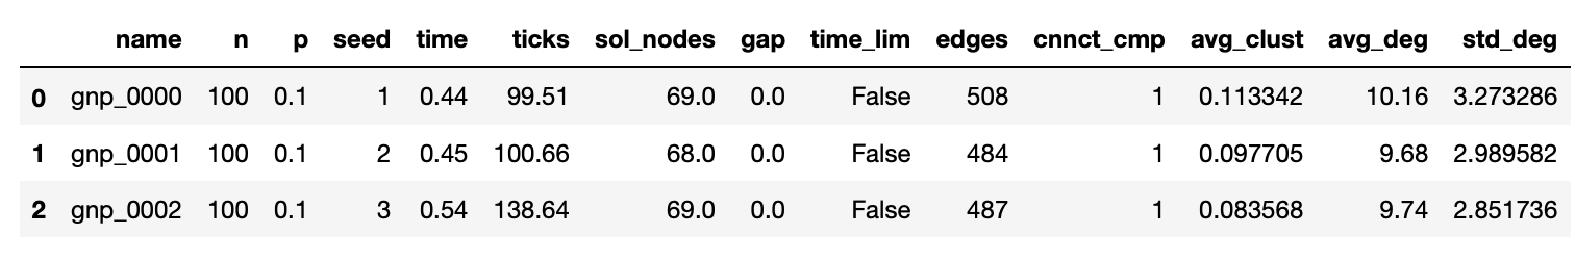
\includegraphics[scale=0.6]{images/csv.eps}
       \caption{Esempio di struttura di un file CSV contenente i risultati della risoluzione di tutti i problemi di vertex cover di una certa tipologia di grafi, in questo caso corrispondente ai grafi $G(n,p)$.}
        \label{fig:csv}
\end{figure}

Come si può notare dalla figura precedente, per ognuna delle istanze sono stati salvati diversi dati sulla risoluzione e sul grafo associato al problema di ottimizzazione. 

%Una breve spiegazione di ciascuno di essi è stata riportata in Tabella \ref{tab:par}.
%
%\begin{table}[ht]
%\centering
%\resizebox{\textwidth}{!}{
%\begin{tabular}{|p{0.35\linewidth} | p{0.6\linewidth}|}
%\hline
%\textsf{name} & codice univoco associato a ciascuna delle istanze di grafo generate\\
%\hline
%\textsf{parametri generazione del grafo}& combinazione dei parametri con cui è stata generata l'istanza di grafo; a diverse tipologie di grafo corrispondono diversi insiemi di parametri\\
%\hline
%\textsf{seed} & seme random utilizzato nella generazione del grafo\\
%\hline
%\textsf{time} & tempo impiegato dal risolutore a trovare una soluzione ottima o, in alternativa, il TIME\_LIMIT imposto\\
%\hline
%\textsf{ticks} & misura effettuata da CPLEX di quanto il risolutore ha impiegato a risolvere l'istanza del problema\\
%\hline
%\textsf{sol\_nodes} & cardinalità del vertex cover individuato, che corrisponde al valore della funzione obiettivo al termine dell'ultima iterazione\\
%\hline
%\textsf{gap} & gap di ottimalità tra soluzione trovata e lower bound al valore della soluzione\\
%\hline
%\textsf{time\_limit} & valore booleano che specifica se il risolutore è andato in TIME\_LIMIT o meno\\
%\hline
%\textsf{edges} & numero di archi dell'istanza di grafo\\
%\hline
%\textsf{cnnct\_cmp} & numero di componenti connesse dell'istanza di grafo\\
%\hline
%\textsf{avg\_clust} & indice di clustering globale medio del grafo\\
%\hline
%\textsf{avg\_deg} & grado medio dei nodi del grafo \\
%\hline
%\textsf{std\_deg} & deviazione standard tra i gradi dei nodi del grafo \\
%\hline
%\end{tabular}}
%\caption{Informazioni estratte per ogni istanza di problema di vertex cover risolta.} 
%\label{tab:par}
%\end{table} 

L'analisi dei dati estratti è stata infine svolta con il supporto di un Jupyter Notebook \cite{jupyter}, applicazione web open-source che permette di coniugare in un unico documento testo ed esecuzione di codice. 


